% Options for packages loaded elsewhere
\PassOptionsToPackage{unicode}{hyperref}
\PassOptionsToPackage{hyphens}{url}
%
\documentclass[
  12pt,
]{article}
\usepackage{amsmath,amssymb}
\usepackage{iftex}
\ifPDFTeX
  \usepackage[T1]{fontenc}
  \usepackage[utf8]{inputenc}
  \usepackage{textcomp} % provide euro and other symbols
\else % if luatex or xetex
  \usepackage{unicode-math} % this also loads fontspec
  \defaultfontfeatures{Scale=MatchLowercase}
  \defaultfontfeatures[\rmfamily]{Ligatures=TeX,Scale=1}
\fi
\usepackage{lmodern}
\ifPDFTeX\else
  % xetex/luatex font selection
    \setmainfont[]{Times New Roman}
\fi
% Use upquote if available, for straight quotes in verbatim environments
\IfFileExists{upquote.sty}{\usepackage{upquote}}{}
\IfFileExists{microtype.sty}{% use microtype if available
  \usepackage[]{microtype}
  \UseMicrotypeSet[protrusion]{basicmath} % disable protrusion for tt fonts
}{}
\makeatletter
\@ifundefined{KOMAClassName}{% if non-KOMA class
  \IfFileExists{parskip.sty}{%
    \usepackage{parskip}
  }{% else
    \setlength{\parindent}{0pt}
    \setlength{\parskip}{6pt plus 2pt minus 1pt}}
}{% if KOMA class
  \KOMAoptions{parskip=half}}
\makeatother
\usepackage{xcolor}
\usepackage[margin=1in]{geometry}
\usepackage{color}
\usepackage{fancyvrb}
\newcommand{\VerbBar}{|}
\newcommand{\VERB}{\Verb[commandchars=\\\{\}]}
\DefineVerbatimEnvironment{Highlighting}{Verbatim}{commandchars=\\\{\}}
% Add ',fontsize=\small' for more characters per line
\usepackage{framed}
\definecolor{shadecolor}{RGB}{248,248,248}
\newenvironment{Shaded}{\begin{snugshade}}{\end{snugshade}}
\newcommand{\AlertTok}[1]{\textcolor[rgb]{0.94,0.16,0.16}{#1}}
\newcommand{\AnnotationTok}[1]{\textcolor[rgb]{0.56,0.35,0.01}{\textbf{\textit{#1}}}}
\newcommand{\AttributeTok}[1]{\textcolor[rgb]{0.13,0.29,0.53}{#1}}
\newcommand{\BaseNTok}[1]{\textcolor[rgb]{0.00,0.00,0.81}{#1}}
\newcommand{\BuiltInTok}[1]{#1}
\newcommand{\CharTok}[1]{\textcolor[rgb]{0.31,0.60,0.02}{#1}}
\newcommand{\CommentTok}[1]{\textcolor[rgb]{0.56,0.35,0.01}{\textit{#1}}}
\newcommand{\CommentVarTok}[1]{\textcolor[rgb]{0.56,0.35,0.01}{\textbf{\textit{#1}}}}
\newcommand{\ConstantTok}[1]{\textcolor[rgb]{0.56,0.35,0.01}{#1}}
\newcommand{\ControlFlowTok}[1]{\textcolor[rgb]{0.13,0.29,0.53}{\textbf{#1}}}
\newcommand{\DataTypeTok}[1]{\textcolor[rgb]{0.13,0.29,0.53}{#1}}
\newcommand{\DecValTok}[1]{\textcolor[rgb]{0.00,0.00,0.81}{#1}}
\newcommand{\DocumentationTok}[1]{\textcolor[rgb]{0.56,0.35,0.01}{\textbf{\textit{#1}}}}
\newcommand{\ErrorTok}[1]{\textcolor[rgb]{0.64,0.00,0.00}{\textbf{#1}}}
\newcommand{\ExtensionTok}[1]{#1}
\newcommand{\FloatTok}[1]{\textcolor[rgb]{0.00,0.00,0.81}{#1}}
\newcommand{\FunctionTok}[1]{\textcolor[rgb]{0.13,0.29,0.53}{\textbf{#1}}}
\newcommand{\ImportTok}[1]{#1}
\newcommand{\InformationTok}[1]{\textcolor[rgb]{0.56,0.35,0.01}{\textbf{\textit{#1}}}}
\newcommand{\KeywordTok}[1]{\textcolor[rgb]{0.13,0.29,0.53}{\textbf{#1}}}
\newcommand{\NormalTok}[1]{#1}
\newcommand{\OperatorTok}[1]{\textcolor[rgb]{0.81,0.36,0.00}{\textbf{#1}}}
\newcommand{\OtherTok}[1]{\textcolor[rgb]{0.56,0.35,0.01}{#1}}
\newcommand{\PreprocessorTok}[1]{\textcolor[rgb]{0.56,0.35,0.01}{\textit{#1}}}
\newcommand{\RegionMarkerTok}[1]{#1}
\newcommand{\SpecialCharTok}[1]{\textcolor[rgb]{0.81,0.36,0.00}{\textbf{#1}}}
\newcommand{\SpecialStringTok}[1]{\textcolor[rgb]{0.31,0.60,0.02}{#1}}
\newcommand{\StringTok}[1]{\textcolor[rgb]{0.31,0.60,0.02}{#1}}
\newcommand{\VariableTok}[1]{\textcolor[rgb]{0.00,0.00,0.00}{#1}}
\newcommand{\VerbatimStringTok}[1]{\textcolor[rgb]{0.31,0.60,0.02}{#1}}
\newcommand{\WarningTok}[1]{\textcolor[rgb]{0.56,0.35,0.01}{\textbf{\textit{#1}}}}
\usepackage{longtable,booktabs,array}
\usepackage{calc} % for calculating minipage widths
% Correct order of tables after \paragraph or \subparagraph
\usepackage{etoolbox}
\makeatletter
\patchcmd\longtable{\par}{\if@noskipsec\mbox{}\fi\par}{}{}
\makeatother
% Allow footnotes in longtable head/foot
\IfFileExists{footnotehyper.sty}{\usepackage{footnotehyper}}{\usepackage{footnote}}
\makesavenoteenv{longtable}
\usepackage{graphicx}
\makeatletter
\def\maxwidth{\ifdim\Gin@nat@width>\linewidth\linewidth\else\Gin@nat@width\fi}
\def\maxheight{\ifdim\Gin@nat@height>\textheight\textheight\else\Gin@nat@height\fi}
\makeatother
% Scale images if necessary, so that they will not overflow the page
% margins by default, and it is still possible to overwrite the defaults
% using explicit options in \includegraphics[width, height, ...]{}
\setkeys{Gin}{width=\maxwidth,height=\maxheight,keepaspectratio}
% Set default figure placement to htbp
\makeatletter
\def\fps@figure{htbp}
\makeatother
\setlength{\emergencystretch}{3em} % prevent overfull lines
\providecommand{\tightlist}{%
  \setlength{\itemsep}{0pt}\setlength{\parskip}{0pt}}
\setcounter{secnumdepth}{5}
% definitions for citeproc citations
\NewDocumentCommand\citeproctext{}{}
\NewDocumentCommand\citeproc{mm}{%
  \begingroup\def\citeproctext{#2}\cite{#1}\endgroup}
\makeatletter
 % allow citations to break across lines
 \let\@cite@ofmt\@firstofone
 % avoid brackets around text for \cite:
 \def\@biblabel#1{}
 \def\@cite#1#2{{#1\if@tempswa , #2\fi}}
\makeatother
\newlength{\cslhangindent}
\setlength{\cslhangindent}{1.5em}
\newlength{\csllabelwidth}
\setlength{\csllabelwidth}{3em}
\newenvironment{CSLReferences}[2] % #1 hanging-indent, #2 entry-spacing
 {\begin{list}{}{%
  \setlength{\itemindent}{0pt}
  \setlength{\leftmargin}{0pt}
  \setlength{\parsep}{0pt}
  % turn on hanging indent if param 1 is 1
  \ifodd #1
   \setlength{\leftmargin}{\cslhangindent}
   \setlength{\itemindent}{-1\cslhangindent}
  \fi
  % set entry spacing
  \setlength{\itemsep}{#2\baselineskip}}}
 {\end{list}}
\usepackage{calc}
\newcommand{\CSLBlock}[1]{\hfill\break\parbox[t]{\linewidth}{\strut\ignorespaces#1\strut}}
\newcommand{\CSLLeftMargin}[1]{\parbox[t]{\csllabelwidth}{\strut#1\strut}}
\newcommand{\CSLRightInline}[1]{\parbox[t]{\linewidth - \csllabelwidth}{\strut#1\strut}}
\newcommand{\CSLIndent}[1]{\hspace{\cslhangindent}#1}
\usepackage{tcolorbox}
\usepackage{amssymb}
\usepackage{yfonts}
\usepackage{bm}
\usepackage{titlesec}
\usepackage{kbordermatrix}


\newtcolorbox{greybox}{
  colback=white,
  colframe=blue,
  coltext=black,
  boxsep=5pt,
  arc=4pt}
  
\newcommand{\sectionbreak}{\clearpage}

 
\newcommand{\ds}[4]{\sum_{{#1}=1}^{#3}\sum_{{#2}=1}^{#4}}
\newcommand{\us}[3]{\mathop{\sum\sum}_{1\leq{#2}<{#1}\leq{#3}}}

\newcommand{\ol}[1]{\overline{#1}}
\newcommand{\ul}[1]{\underline{#1}}

\newcommand{\amin}[1]{\mathop{\text{argmin}}_{#1}}
\newcommand{\amax}[1]{\mathop{\text{argmax}}_{#1}}

\newcommand{\ci}{\perp\!\!\!\perp}

\newcommand{\mc}[1]{\mathcal{#1}}
\newcommand{\mb}[1]{\mathbb{#1}}
\newcommand{\mf}[1]{\mathfrak{#1}}

\newcommand{\eps}{\epsilon}
\newcommand{\lbd}{\lambda}
\newcommand{\alp}{\alpha}
\newcommand{\df}{=:}
\newcommand{\am}[1]{\mathop{\text{argmin}}_{#1}}
\newcommand{\ls}[2]{\mathop{\sum\sum}_{#1}^{#2}}
\newcommand{\ijs}{\mathop{\sum\sum}_{1\leq i<j\leq n}}
\newcommand{\jis}{\mathop{\sum\sum}_{1\leq j<i\leq n}}
\newcommand{\sij}{\sum_{i=1}^n\sum_{j=1}^n}
	
\ifLuaTeX
  \usepackage{selnolig}  % disable illegal ligatures
\fi
\usepackage{bookmark}
\IfFileExists{xurl.sty}{\usepackage{xurl}}{} % add URL line breaks if available
\urlstyle{same}
\hypersetup{
  pdfauthor={Jan de Leeuw - University of California Los Angeles},
  hidelinks,
  pdfcreator={LaTeX via pandoc}}

\title{Smacof at 50: A Manual\\
Part 2: smacofAC: Metric and Interval Smacof}
\author{Jan de Leeuw - University of California Los Angeles}
\date{Started December 12 2022, Version of May 28, 2024}

\begin{document}
\maketitle

{
\setcounter{tocdepth}{3}
\tableofcontents
}
\textbf{Note:} This is a working manuscript which will be expanded/updated
frequently. All suggestions for improvement are welcome. All Rmd, tex,
html, pdf, R, and C files are in the public domain. Attribution will be
appreciated, but is not required. All files can be found at
\url{https://github.com/deleeuw} in the smacofAC directories of the repositories smacofCode, smacofManual, and smacofExamples.

\section{Introduction}\label{introduction}

In this part of the manual we discuss metric MDS, and the program
smacofAC. Metric MDS is the core of all smacof programs, because they
all have the majorization algorithm based on the Guttman transform
in common.

There are two options, \emph{bounds} and \emph{constant}, to make smacofAC more widely applicable. Using these options the metric MDS problem becomes minimization of
\begin{equation}
\sigma(X,\hat D)=\sum\sum w_{ij}(\hat d_{ij}-d_{ij}(X))^2
\label{eq:sdefac}
\end{equation}
over both \(X\) and \(\hat D\), allowing some limited ``metric'' transformations of the data \(\Delta\). Here \(\Delta^-\) and \(\Delta^+\) are known matrices with bounds, and \(c\) is an unknown additive constant. The four ``metric'' types of transformations
relating disparities \(\hat d_{ij}\) to dissimilarities \(\delta_{ij}\) are

\begin{enumerate}
\def\labelenumi{\arabic{enumi}.}
\tightlist
\item
  type AC1: if bounds = 0 and constant = 0 \(\hat d_{ij}=\delta_{ij}\).
\item
  type AC2: if bounds = 0 and constant = 1 \(\hat d_{ij}=\delta_{ij}+c\) for some \(c\),
\item
  type AC3: if bounds = 1 and constant = 0 \(\delta^-_{ij}\leq\hat d_{ij}\leq\delta^+_{ij}\),
\item
  type AC4: if bounds = 1 and constant = 1 \(\delta^-_{ij}+c\leq\hat d_{ij}\leq\delta^+_{ij}+c\) for some \(c\),
\end{enumerate}

All four types of transformations also require that \(\hat d_{ij}\geq 0\) for all \((i,j)\). There are extensions of the smacof theory (Heiser (1991)) that do not require non-negativity of the disparities, but in the implementations in this manual we always force them to be non-negative. Note that AC3 is AC4 with \(c=0\) and AC2 is AC4 with \(\Delta^-=\Delta^+=\Delta\).

Note that for types AC2 and AC4 the data \(\Delta\) do not need to be non-negative. In fact,
the original motivation for the additive constant in classical scaling (Messick and Abelson (1956))
was that Thurstonian analysis of tetrad or triad comparisons produced dissimilarities on an interval scale, and thus could very well include negative values.

In AC3 and AC4 there is no mention of \(\Delta\), which means
the bounds \(\Delta^-\) and \(\Delta^+\) are actually the data. There are several possible uses of the bounds. We could
collect dissimilarity data by asking subjects for interval judgments. Instead
of a rating scale with possible responses from one to ten we could ask
for a mark on a line between zero and ten, and then interpret the
marks as a choice of one of the intervals \([k, k+1]\). These finite precision
or interval type of data could even come from physical measurements of distances.
Thus the bounds parameter provides one way to incorporate uncertainty into MDS, similar to interval analysis, fuzzy computing, or soft computing.

The non-negativity requirement for \(\hat D\) implies bounds for the additive constant
\(c\). In AC2 we need \(c\geq-\min\delta_{ij}\) to maintain non-negativity. For AC4 we must have \(c\geq-\min\delta_{ij}^+\), otherwise the constraints on the transformation are inconsistent.
Clearly for consistency of AC3 and AC4 we require that \(\delta_{ij}^-\leq\delta_{ij}^+\)
for all \((i,j)\). It makes sense in most situations to choose \(\Delta^-\) and \(\Delta^+\)
to be monotone with \(\Delta\), but there is no requirement to do so.

\section{Program}\label{program}

\subsection{Parameters}\label{parameters}

\begin{Shaded}
\begin{Highlighting}[]
\NormalTok{smacofAC }\OtherTok{\textless{}{-}} \ControlFlowTok{function}\NormalTok{(delta,}
                     \AttributeTok{ndim =} \DecValTok{2}\NormalTok{,}
                     \AttributeTok{wmat =} \ConstantTok{NULL}\NormalTok{,}
                     \AttributeTok{xold =} \ConstantTok{NULL}\NormalTok{,}
                     \AttributeTok{bounds =} \ConstantTok{FALSE}\NormalTok{,}
                     \AttributeTok{constant =} \ConstantTok{FALSE}\NormalTok{,}
                     \AttributeTok{deltalw =} \ConstantTok{NULL}\NormalTok{,}
                     \AttributeTok{deltaup =} \ConstantTok{NULL}\NormalTok{,}
                     \AttributeTok{alpha =} \DecValTok{2}\NormalTok{,}
                     \AttributeTok{labels =} \FunctionTok{row.names}\NormalTok{(delta),}
                     \AttributeTok{width =} \DecValTok{15}\NormalTok{,}
                     \AttributeTok{precision =} \DecValTok{10}\NormalTok{,}
                     \AttributeTok{itmax =} \DecValTok{1000}\NormalTok{,}
                     \AttributeTok{eps =} \FloatTok{1e{-}10}\NormalTok{,}
                     \AttributeTok{verbose =} \ConstantTok{TRUE}\NormalTok{,}
                     \AttributeTok{kitmax =} \DecValTok{5}\NormalTok{,}
                     \AttributeTok{keps =} \FloatTok{1e{-}10}\NormalTok{,}
                     \AttributeTok{kverbose =} \ConstantTok{FALSE}\NormalTok{,}
                     \AttributeTok{init =} \DecValTok{1}\NormalTok{)}
\end{Highlighting}
\end{Shaded}

The parameters \emph{constant}, \emph{bounds}, \emph{alpha}, \emph{kitmax}, \emph{kepsi}, and \emph{kverbose} are only relevant for AC2, AC3, and AC4. Nevertheless even for AC1 they should have integer values, it just doesn't matter what these values are.
Parameter \emph{ndim} is the number of dimensions, and \emph{init} tells if an initial configuration
is read from a file (init = 1), is computed using classical scaling (init = 2), or is
a random configuration (init = 3). Parameters
\emph{itmax}, \emph{epsi}, and \emph{verbose} control the iterations. The maximum number of iterations
is \emph{itmax}, the iterations stop if the decrease of stress in an iteration is less than
1E-\emph{epsi}, and if \emph{verbose} is one intermediate iteration results are written to stdout.
These intermediate iteration results are formatted with the R function formatC(), using
\emph{width} for the width argument and \emph{precision} for the digits argument.

\subsection{Algorithm}\label{algorithm}

\subsubsection{Type AC1}\label{type-ac1}

This is standard non-metric smacof, no bells and whistles.

\subsubsection{Type AC2}\label{type-ac2}

For AC2 we also optimize over the additive constant \(c\), and thus the ALS algorithm has two
sub-steps. The first sub-step consists of a number of Guttman iterations to update \(X\) for given
\(\hat D\) (i.e.~for given \(c\)) and the second sub-step updates \(c\) for given \(X\).
Parameters \emph{kitmax}, \emph{kepsi}, and \emph{kverbose} control the inner iterations in the first sub-step in the same way as \emph{itmax}, \emph{epsi}, and \emph{verbose} control the
outer iterations that include both sub-steps. No inner iterations are used
to update the additive constant, which only requires computing a weighted
average.
\begin{equation}
c=-\frac{\sum\sum w_{ij}(\delta_{ij}-d_{ij}(X))}{\sum\sum w_{ij}}
\label{eq:updac2}
\end{equation}
AC2 should give the same results as the MDS method of Cooper (1972).

\subsubsection{Type AC3}\label{type-ac3}

The algorithm for AC3 has the same structure as that for AC2. Instead of
a second sub-step computing the additive constant, the second sub-step
computes \(\hat D\) by squeezing the \(D(X)\) into the bounds. Thus
\begin{equation}
\hat d_{ij}=\begin{cases}
\delta_{ij}^-&\text{ if }d_{ij}(X)<\delta_{ij}^-,\\
\delta_{ij}^+&\text{ if }d_{ij}(X)>\delta_{ij}^+,\\
d_{ij}(X)&\text{ otherwise }.
\end{cases}
\label{eq:updac3}
\end{equation}
Obviously no iterations are required in the second sub-step.

\subsubsection{Type AC4}\label{type-ac4}

Of the four regression problems in the second ALS sub-step only the one for AC4 with both bounds and additive constant is non-trivial. We'll give it some extra attention.

It may help to give an example of what it actually requires. We use the De Gruijter example
with nine Dutch political parties from 1967 (De Gruijter (1967)). For ease of reference we include the data here. Dissimilarities are averages over a group of 100 students from an introductory psychology course.

\begin{verbatim}
##       KVP PvdA  VVD  ARP  CHU  CPN  PSP   BP  D66
## KVP  0.00 5.63 5.27 4.60 4.80 7.54 6.73 7.18 6.17
## PvdA 5.63 0.00 6.72 5.64 6.22 5.12 4.59 7.22 5.47
## VVD  5.27 6.72 0.00 5.46 4.97 8.13 7.55 6.90 4.67
## ARP  4.60 5.64 5.46 0.00 3.20 7.84 6.73 7.28 6.13
## CHU  4.80 6.22 4.97 3.20 0.00 7.80 7.08 6.96 6.04
## CPN  7.54 5.12 8.13 7.84 7.80 0.00 4.08 6.34 7.42
## PSP  6.73 4.59 7.55 6.73 7.08 4.08 0.00 6.88 6.36
## BP   7.18 7.22 6.90 7.28 6.96 6.34 6.88 0.00 7.36
## D66  6.17 5.47 4.67 6.13 6.04 7.42 6.36 7.36 0.00
\end{verbatim}

We compute distances from the Torgerson solution. The Shepard plot for \(c=0\) and the Torgerson distances is in figure \ref{fig:bandplot}. The two blue
lines are connecting the \(\delta_{ij}^-\) and the \(\delta_{ij}^+\), i.e.~they give
the bounds for \(c=0\). In our example the lines are parallel, because \(\delta_{ij}^+-\delta_{ij}^-=2\) for all \((i,j)\), but in general this may not be the case.
The points between the two lines do not contribute to the loss, and
the points outside the band contribute by how much they are outside, as indicated by the
black vertical fitlines.

By varying \(c\) we shift the region between the two parallel lines upwards or downwards. The width of the region, or more generally the shape, always remains the same, because it is determined by the difference of \(\delta^+\) and \(\delta^-\) and does not depend on \(c\). The
optimal \(c\) is that shift for which the red \((\delta_{ij},d_{ij}(X))\) points are as much as possible within the strip between the \(\delta^-\) and \(\delta^+\) lines. This is in the least squares sense, which means that we minimize the horizontal squared distances from the points outside the strip to the \(\delta^-\) and \(\delta^+\) lines (i.e.~the black vertical lines).

Let's formalize this. Define
\begin{equation}
\phi_{ij}(c):=\min_{\delta_{ij}\geq 0}\{(\delta_{ij}-d_{ij}(X))^2\mid \delta^-_{ij}+c\leq\delta_{ij}\leq\delta^+_{ij}+c\}
\label{eq:phiijdef}
\end{equation}
and
\begin{equation}
\phi(c):=\sum\sum w_{ij}\phi_{ij}(c)
\label{eq:phidef}
\end{equation}
The constraints are consistent if \(\delta_{ij}^++c\geq 0\), i.e.~if \(c\geq c_0:=-\min\delta_{ij}^+\).
The regression problem is to minimize \(\phi\) over \(c\geq c_0:=-\min\delta_{ij}^+\).

Figure has an example of one of the \(\phi_{ij}\). The value of the
\(d_{ij}(X)\) we used is , \(\delta_{ij}\) is , \(\delta_{ij}^-\) is , and \(\delta_{ij}^+\) is .
The two red vertical lines
are at \(c=d_{ij}(X)-\delta_{ij}^+\) and \(c=d_{ij}(X)-\delta_{ij}^-\).

Now
\begin{equation}
\hat d_{ij}=\begin{cases}
\delta_{ij}^-+c&\text{ if }c\geq d_{ij}(X)-\delta_{ij}^-,\\
\delta_{ij}^++c&\text{ if }c\leq d_{ij}(X)-\delta_{ij}^+,\\
d_{ij}(X)&\text{ otherwise}.
\end{cases}
\label{eq:solves}
\end{equation}
and thus
\begin{equation}
\phi_{ij}(c)=\begin{cases}
(d_{ij}(X)-(\delta_{ij}^-+c))^2&\text{ if }c\geq d_{ij}(X)-\delta_{ij}^-,\\
(d_{ij}(X)-(\delta_{ij}^++c))^2&\text{ if }c\leq d_{ij}(X)-\delta_{ij}^+,\\
0&\text{ otherwise}.
\end{cases}
\label{eq:funcs}
\end{equation}
It follows that \(\phi_{ij}\) is
piecewise quadratic, convex, and continuously differentiable. The derivative
is piecewise linear, continuous, and increasing. In fact
\begin{equation}
\mathcal{D}\phi_{ij}(c)=\begin{cases}
2(c-(d_{ij}(X)-\delta_{ij}^-))&\text{ if }c\geq d_{ij}(X)-\delta_{ij}^-,\\
2(c-(d_{ij}(X)-\delta_{ij}^+))&\text{ if }c\leq d_{ij}(X)-\delta_{ij}^+,\\
0&\text{ otherwise}.
\end{cases}
\label{eq:derivs}
\end{equation}

Since \(\phi\) is a positive linear combination of the \(\phi_{ij}\) it is also piecewise quadratic, convex, and continuously differentiable,
with a continuous piecewise linear increasing derivative. Note \(\phi\) is \textbf{not} twice-differentiable
and \textbf{not} strictly convex. Figure \ref{fig:morefunc} has a plot of \(\phi\) for the De Gruijter
example. The red vertical lines are at \(c=c_0\) and at \(c_1:=\max\{d_{ij}(X)-\delta_{ij}^-\}\). From \eqref{eq:derivs} we see that if \(c\geq c_1\)
then \(\mathcal{D}\phi(c_1)\geq 0\) and thus we can look for the optimum \(c\) in the interval
\([c_0,c_1]\).

We minimize \(\phi\) by using the R function optimize().

\subsection{Output}\label{output}

\subsection{Plots}\label{plots}

\section{Examples}\label{examples}

\subsection{De Gruijter (1967)}\label{degruijter_67}

It may help to give an example of what it actually requires. We use the De Gruijter example
with nine Dutch political parties from 1967 (De Gruijter (1967)). Dissimilarities are averages over a group of 100 students from an introductory psychology course.

We compute optimal
solutions for all four types AC1-AC4 (two dimensions, Torgerson initial estimate,
no weights). We iterate until the difference in consecutive stress values is
less than 1e-10. For each of the four runs we give the number of iterations,
the final stress, and the additive constant in case of AC2 and AC4. We also
make three plots: the Shepard plot with points \((\delta_{ij},d_{ij}(X))\)
in blue and with points \((\delta_{ij},\hat d_{ij})\) in red, the configuration
plot with a labeled \(X\), and the dist-dhat plot with points \((d_{ij}(X),\hat d_{ij})\)
scattered around the line \(d=\hat d\). Line segments are drawn in the plots to
show the fit of all pairs \((i,j)\).

\subsection{Type AC1}\label{type-ac1-1}

\begin{center}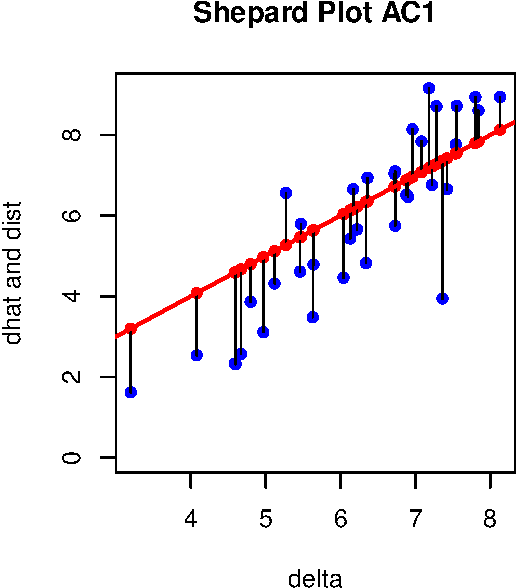
\includegraphics{smacofAC_files/figure-latex/gruijterh00-1} \end{center}

\begin{center}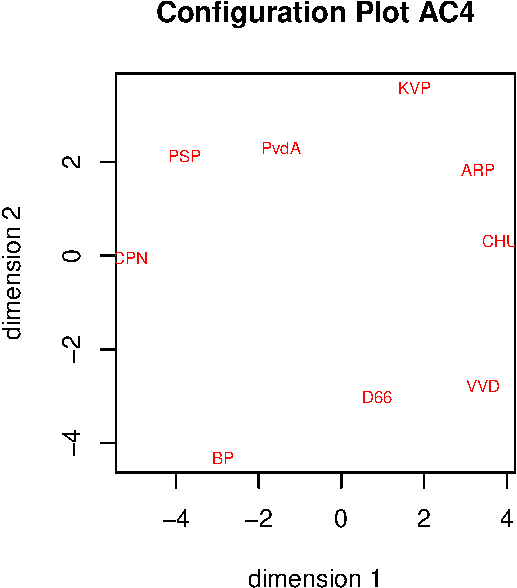
\includegraphics{smacofAC_files/figure-latex/gruijterh00-2} \end{center}

For AC1 we find a minimum stress of 32.2208145 after 112 iterations.
The Shepard plot has a substantial intercept, which suggest that an additive
constant may improve the fit. This is typical for average similarity judgments
over heterogeneous groups of individuals. It is the reason why Ekman (1954)
linearly transformed his average similarities so that the smallest became zero
and the largest became one. That amounts to applying the additive constant before
the MDS analysis.

To give some content to the configuration plot: CPN (communists), PSP (pacifists),
and PvdA (social democrats) are leftists parties, ARP (protestants), CHU (other
protestants), KVP (catholics) are religious parties, BP (farmers) is a
right-wing protest party, VVD (classical liberals) is a conservative party, and D'66
(pragmatists, centrists) was brand new in 1967 and was supposedly beyond left and right.

\subsection{Type AC2}\label{type-ac2-1}

\begin{center}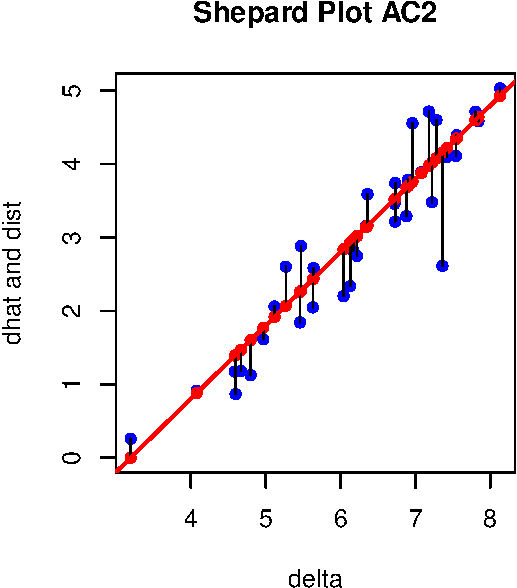
\includegraphics{smacofAC_files/figure-latex/gruijterh10-1} \end{center}

\begin{center}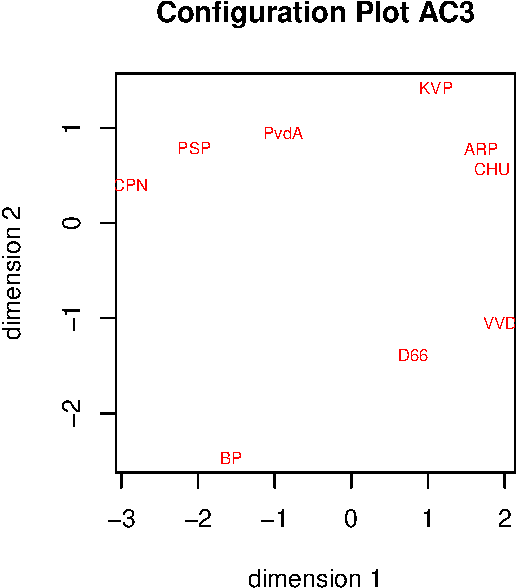
\includegraphics{smacofAC_files/figure-latex/gruijterh10-2} \end{center}

As expected, the additive constant improves the fit. We have convergence after 25
iterations to stress 3.6661492. The additive constant is -3.2, which means the smallest \(\delta_{ij}+c\), between ARP and CHU, is now zero. The configuration shows the same three groups, but they cluster a bit more tightly. This is to be expected. Without the
additive constant the dissimilarities are more equal and consequently the distances are
more equal to. The configuration tends more to what we see if all dissimilarities are equal,
i.e.~to points regularly spaced on a circle (De Leeuw and Stoop (1984)).

\subsection{Type AC3}\label{type-ac3-1}

\begin{verbatim}
## itel  1 sold    97.4130852810 smid    41.9550246691 snew     8.4543139218 
## itel  2 sold     8.4543139218 smid     7.4098292411 snew     6.6451369923 
## itel  3 sold     6.6451369923 smid     5.8490240542 snew     5.2489286201 
## itel  4 sold     5.2489286201 smid     4.6072125696 snew     4.1502164078 
## itel  5 sold     4.1502164078 smid     3.6168200275 snew     3.2322363271 
## itel  6 sold     3.2322363271 smid     2.7379930587 snew     2.4414269275 
## itel  7 sold     2.4414269275 smid     2.1593556178 snew     1.9752760141 
## itel  8 sold     1.9752760141 smid     1.8092882729 snew     1.6764432789 
## itel  9 sold     1.6764432789 smid     1.5582549338 snew     1.4557443279 
## itel  10 sold     1.4557443279 smid     1.3629036613 snew     1.2793695305 
## itel  11 sold     1.2793695305 smid     1.2025292754 snew     1.1324574520 
## itel  12 sold     1.1324574520 smid     1.0674066563 snew     1.0078467610 
## itel  13 sold     1.0078467610 smid     0.9522276636 snew     0.9013064460 
## itel  14 sold     0.9013064460 smid     0.8535746120 snew     0.8098200136 
## itel  15 sold     0.8098200136 smid     0.7685362919 snew     0.7305939018 
## itel  16 sold     0.7305939018 smid     0.6945836967 snew     0.6615054424 
## itel  17 sold     0.6615054424 smid     0.6300498204 snew     0.6011559114 
## itel  18 sold     0.6011559114 smid     0.5735956560 snew     0.5483309878 
## itel  19 sold     0.5483309878 smid     0.5241981027 snew     0.5020869304 
## itel  20 sold     0.5020869304 smid     0.4809112562 snew     0.4614299495 
## itel  21 sold     0.4614299495 smid     0.4425815492 snew     0.4251667367 
## itel  22 sold     0.4251667367 smid     0.4082440772 snew     0.3925990995 
## itel  23 sold     0.3925990995 smid     0.3773608282 snew     0.3632632528 
## itel  24 sold     0.3632632528 smid     0.3494646668 snew     0.3366780605 
## itel  25 sold     0.3366780605 smid     0.3241244799 snew     0.3124866156 
## itel  26 sold     0.3124866156 smid     0.3010402505 snew     0.2904279430 
## itel  27 sold     0.2904279430 smid     0.2799638410 snew     0.2702326078 
## itel  28 sold     0.2702326078 smid     0.2606115288 snew     0.2516575222 
## itel  29 sold     0.2516575222 smid     0.2427970344 snew     0.2345497021 
## itel  30 sold     0.2345497021 smid     0.2263873344 snew     0.2187862641 
## itel  31 sold     0.2187862641 smid     0.2112642137 snew     0.2042558938 
## itel  32 sold     0.2042558938 smid     0.1973219792 snew     0.1908667641 
## itel  33 sold     0.1908667641 smid     0.1844985022 snew     0.1785576365 
## itel  34 sold     0.1785576365 smid     0.1726814275 snew     0.1672223800 
## itel  35 sold     0.1672223800 smid     0.1618749397 snew     0.1568871640 
## itel  36 sold     0.1568871640 smid     0.1520054971 snew     0.1474133814 
## itel  37 sold     0.1474133814 smid     0.1429220273 snew     0.1386839988 
## itel  38 sold     0.1386839988 smid     0.1345340757 snew     0.1306172696 
## itel  39 sold     0.1306172696 smid     0.1267823207 snew     0.1231570280 
## itel  40 sold     0.1231570280 smid     0.1195991686 snew     0.1162371624 
## itel  41 sold     0.1162371624 smid     0.1129422950 snew     0.1098197491 
## itel  42 sold     0.1098197491 smid     0.1067564820 snew     0.1038529288 
## itel  43 sold     0.1038529288 smid     0.1009986094 snew     0.0982958229 
## itel  44 sold     0.0982958229 smid     0.0956394236 snew     0.0931205429 
## itel  45 sold     0.0931205429 smid     0.0906400571 snew     0.0882903384 
## itel  46 sold     0.0882903384 smid     0.0859714475 snew     0.0837774185 
## itel  47 sold     0.0837774185 smid     0.0816103623 snew     0.0795595988 
## itel  48 sold     0.0795595988 smid     0.0775350522 snew     0.0756158480 
## itel  49 sold     0.0756158480 smid     0.0737069060 snew     0.0718997892 
## itel  50 sold     0.0718997892 smid     0.0700922565 snew     0.0683803581 
## itel  51 sold     0.0683803581 smid     0.0666579412 snew     0.0650295657 
## itel  52 sold     0.0650295657 smid     0.0633889911 snew     0.0618371988 
## itel  53 sold     0.0618371988 smid     0.0602695635 snew     0.0587893711 
## itel  54 sold     0.0587893711 smid     0.0572852862 snew     0.0558726314 
## itel  55 sold     0.0558726314 smid     0.0544335762 snew     0.0530845479 
## itel  56 sold     0.0530845479 smid     0.0517076720 snew     0.0504187686 
## itel  57 sold     0.0504187686 smid     0.0490986716 snew     0.0478667578 
## itel  58 sold     0.0478667578 smid     0.0466025175 snew     0.0454246636 
## itel  59 sold     0.0454246636 smid     0.0442126511 snew     0.0430859071 
## itel  60 sold     0.0430859071 smid     0.0419238186 snew     0.0408458015 
## itel  61 sold     0.0408458015 smid     0.0397344293 snew     0.0387034342 
## itel  62 sold     0.0387034342 smid     0.0376390715 snew     0.0366529538 
## itel  63 sold     0.0366529538 smid     0.0356351002 snew     0.0346922685 
## itel  64 sold     0.0346922685 smid     0.0337172756 snew     0.0328162870 
## itel  65 sold     0.0328162870 smid     0.0318859969 snew     0.0310252529 
## itel  66 sold     0.0310252529 smid     0.0301365454 snew     0.0293146845 
## itel  67 sold     0.0293146845 smid     0.0284661882 snew     0.0276818686 
## itel  68 sold     0.0276818686 smid     0.0268736638 snew     0.0261255295 
## itel  69 sold     0.0261255295 smid     0.0253515999 snew     0.0246386243 
## itel  70 sold     0.0246386243 smid     0.0239018541 snew     0.0232227235 
## itel  71 sold     0.0232227235 smid     0.0225233461 snew     0.0218768243 
## itel  72 sold     0.0218768243 smid     0.0212105688 snew     0.0205956586 
## itel  73 sold     0.0205956586 smid     0.0199609330 snew     0.0193766033 
## itel  74 sold     0.0193766033 smid     0.0187743001 snew     0.0182194345 
## itel  75 sold     0.0182194345 smid     0.0176476992 snew     0.0171212966 
## itel  76 sold     0.0171212966 smid     0.0165791103 snew     0.0160801664 
## itel  77 sold     0.0160801664 smid     0.0155665396 snew     0.0150940641 
## itel  78 sold     0.0150940641 smid     0.0146080603 snew     0.0141610730 
## itel  79 sold     0.0141610730 smid     0.0137017748 snew     0.0132793044 
## itel  80 sold     0.0132793044 smid     0.0128460418 snew     0.0124471117 
## itel  81 sold     0.0124471117 smid     0.0120383862 snew     0.0116620659 
## itel  82 sold     0.0116620659 smid     0.0112774626 snew     0.0109227851 
## itel  83 sold     0.0109227851 smid     0.0105587161 snew     0.0102248820 
## itel  84 sold     0.0102248820 smid     0.0098838778 snew     0.0095698425 
## itel  85 sold     0.0095698425 smid     0.0092487574 snew     0.0089536963 
## itel  86 sold     0.0089536963 smid     0.0086521341 snew     0.0083751510 
## itel  87 sold     0.0083751510 smid     0.0080919781 snew     0.0078322169 
## itel  88 sold     0.0078322169 smid     0.0075666147 snew     0.0073232264 
## itel  89 sold     0.0073232264 smid     0.0070742856 snew     0.0068464430 
## itel  90 sold     0.0068464430 smid     0.0066132474 snew     0.0064001456 
## itel  91 sold     0.0064001456 smid     0.0061817952 snew     0.0059826528 
## itel  92 sold     0.0059826528 smid     0.0057802663 snew     0.0055942116 
## itel  93 sold     0.0055942116 smid     0.0054047931 snew     0.0052311501 
## itel  94 sold     0.0052311501 smid     0.0050539660 snew     0.0048920336 
## itel  95 sold     0.0048920336 smid     0.0047266122 snew     0.0045756432 
## itel  96 sold     0.0045756432 smid     0.0044211081 snew     0.0042792136 
## itel  97 sold     0.0042792136 smid     0.0041326493 snew     0.0039985613 
## itel  98 sold     0.0039985613 smid     0.0038606482 snew     0.0037337299 
## itel  99 sold     0.0037337299 smid     0.0036026143 snew     0.0034825438 
## itel  100 sold     0.0034825438 smid     0.0033580833 snew     0.0032445924 
## itel  101 sold     0.0032445924 smid     0.0031268398 snew     0.0030196948 
## itel  102 sold     0.0030196948 smid     0.0029084545 snew     0.0028074476 
## itel  103 sold     0.0028074476 smid     0.0027025336 snew     0.0026074631 
## itel  104 sold     0.0026074631 smid     0.0025086875 snew     0.0024193512 
## itel  105 sold     0.0024193512 smid     0.0023262643 snew     0.0022424654 
## itel  106 sold     0.0022424654 smid     0.0021553797 snew     0.0020768877 
## itel  107 sold     0.0020768877 smid     0.0019953227 snew     0.0019219223 
## itel  108 sold     0.0019219223 smid     0.0018458400 snew     0.0017772963 
## itel  109 sold     0.0017772963 smid     0.0017057245 snew     0.0016446713 
## itel  110 sold     0.0016446713 smid     0.0015838944 snew     0.0015303032 
## itel  111 sold     0.0015303032 smid     0.0014763882 snew     0.0014277542 
## itel  112 sold     0.0014277542 smid     0.0013787501 snew     0.0013340577 
## itel  113 sold     0.0013340577 smid     0.0012890894 snew     0.0012477951 
## itel  114 sold     0.0012477951 smid     0.0012064204 snew     0.0011681595 
## itel  115 sold     0.0011681595 smid     0.0011299951 snew     0.0010944827 
## itel  116 sold     0.0010944827 smid     0.0010585786 snew     0.0010256055 
## itel  117 sold     0.0010256055 smid     0.0009925089 snew     0.0009618597 
## itel  118 sold     0.0009618597 smid     0.0009313870 snew     0.0009028660 
## itel  119 sold     0.0009028660 smid     0.0008742102 snew     0.0008476717 
## itel  120 sold     0.0008476717 smid     0.0008210857 snew     0.0007963649 
## itel  121 sold     0.0007963649 smid     0.0007716538 snew     0.0007485214 
## itel  122 sold     0.0007485214 smid     0.0007255726 snew     0.0007038565 
## itel  123 sold     0.0007038565 smid     0.0006822460 snew     0.0006618474 
## itel  124 sold     0.0006618474 smid     0.0006414818 snew     0.0006223115 
## itel  125 sold     0.0006223115 smid     0.0006031260 snew     0.0005851042 
## itel  126 sold     0.0005851042 smid     0.0005670511 snew     0.0005501055 
## itel  127 sold     0.0005501055 smid     0.0005331016 snew     0.0005171660 
## itel  128 sold     0.0005171660 smid     0.0005012225 snew     0.0004862336 
## itel  129 sold     0.0004862336 smid     0.0004712550 snew     0.0004571555 
## itel  130 sold     0.0004571555 smid     0.0004430868 snew     0.0004298229 
## itel  131 sold     0.0004298229 smid     0.0004166114 snew     0.0004041327 
## itel  132 sold     0.0004041327 smid     0.0003917278 snew     0.0003799870 
## itel  133 sold     0.0003799870 smid     0.0003683391 snew     0.0003572921 
## itel  134 sold     0.0003572921 smid     0.0003463530 snew     0.0003359581 
## itel  135 sold     0.0003359581 smid     0.0003256809 snew     0.0003158995 
## itel  136 sold     0.0003158995 smid     0.0003062400 snew     0.0002970358 
## itel  137 sold     0.0002970358 smid     0.0002879569 snew     0.0002792959 
## itel  138 sold     0.0002792959 smid     0.0002707632 snew     0.0002626133 
## itel  139 sold     0.0002626133 smid     0.0002545945 snew     0.0002469255 
## itel  140 sold     0.0002469255 smid     0.0002393903 snew     0.0002321738 
## itel  141 sold     0.0002321738 smid     0.0002250933 snew     0.0002183027 
## itel  142 sold     0.0002183027 smid     0.0002116497 snew     0.0002052599 
## itel  143 sold     0.0002052599 smid     0.0001990090 snew     0.0001929963 
## itel  144 sold     0.0001929963 smid     0.0001871232 snew     0.0001814652 
## itel  145 sold     0.0001814652 smid     0.0001756810 snew     0.0001703685 
## itel  146 sold     0.0001703685 smid     0.0001649346 snew     0.0001599422 
## itel  147 sold     0.0001599422 smid     0.0001548371 snew     0.0001501463 
## itel  148 sold     0.0001501463 smid     0.0001453494 snew     0.0001409426 
## itel  149 sold     0.0001409426 smid     0.0001364348 snew     0.0001322952 
## itel  150 sold     0.0001322952 smid     0.0001280586 snew     0.0001241703 
## itel  151 sold     0.0001241703 smid     0.0001201882 snew     0.0001165364 
## itel  152 sold     0.0001165364 smid     0.0001127934 snew     0.0001093639 
## itel  153 sold     0.0001093639 smid     0.0001058460 snew     0.0001026255 
## itel  154 sold     0.0001026255 smid     0.0000993192 snew     0.0000962953 
## itel  155 sold     0.0000962953 smid     0.0000931880 snew     0.0000903490 
## itel  156 sold     0.0000903490 smid     0.0000874289 snew     0.0000847637 
## itel  157 sold     0.0000847637 smid     0.0000820194 snew     0.0000795176 
## itel  158 sold     0.0000795176 smid     0.0000769388 snew     0.0000745906 
## itel  159 sold     0.0000745906 smid     0.0000721671 snew     0.0000699633 
## itel  160 sold     0.0000699633 smid     0.0000676859 snew     0.0000656178 
## itel  161 sold     0.0000656178 smid     0.0000634777 snew     0.0000615371 
## itel  162 sold     0.0000615371 smid     0.0000595259 snew     0.0000577052 
## itel  163 sold     0.0000577052 smid     0.0000558151 snew     0.0000541071 
## itel  164 sold     0.0000541071 smid     0.0000523308 snew     0.0000507287 
## itel  165 sold     0.0000507287 smid     0.0000490594 snew     0.0000475568 
## itel  166 sold     0.0000475568 smid     0.0000459880 snew     0.0000445788 
## itel  167 sold     0.0000445788 smid     0.0000431046 snew     0.0000417832 
## itel  168 sold     0.0000417832 smid     0.0000403977 snew     0.0000391588 
## itel  169 sold     0.0000391588 smid     0.0000379805 snew     0.0000368139 
## itel  170 sold     0.0000368139 smid     0.0000357070 snew     0.0000346100 
## itel  171 sold     0.0000346100 smid     0.0000335698 snew     0.0000325382 
## itel  172 sold     0.0000325382 smid     0.0000315605 snew     0.0000305904 
## itel  173 sold     0.0000305904 smid     0.0000296716 snew     0.0000287591 
## itel  174 sold     0.0000287591 smid     0.0000278957 snew     0.0000270375 
## itel  175 sold     0.0000270375 smid     0.0000262261 snew     0.0000254189 
## itel  176 sold     0.0000254189 smid     0.0000246563 snew     0.0000238972 
## itel  177 sold     0.0000238972 smid     0.0000231804 snew     0.0000224647 
## itel  178 sold     0.0000224647 smid     0.0000217632 snew     0.0000210923 
## itel  179 sold     0.0000210923 smid     0.0000204335 snew     0.0000198033 
## itel  180 sold     0.0000198033 smid     0.0000191846 snew     0.0000185926 
## itel  181 sold     0.0000185926 smid     0.0000180116 snew     0.0000174556 
## itel  182 sold     0.0000174556 smid     0.0000169099 snew     0.0000163878 
## itel  183 sold     0.0000163878 smid     0.0000158752 snew     0.0000153849 
## itel  184 sold     0.0000153849 smid     0.0000149035 snew     0.0000144430 
## itel  185 sold     0.0000144430 smid     0.0000139910 snew     0.0000135586 
## itel  186 sold     0.0000135586 smid     0.0000131340 snew     0.0000127280 
## itel  187 sold     0.0000127280 smid     0.0000123292 snew     0.0000119480 
## itel  188 sold     0.0000119480 smid     0.0000115735 snew     0.0000112155 
## itel  189 sold     0.0000112155 smid     0.0000108639 snew     0.0000105277 
## itel  190 sold     0.0000105277 smid     0.0000101975 snew     0.0000098819 
## itel  191 sold     0.0000098819 smid     0.0000095718 snew     0.0000092755 
## itel  192 sold     0.0000092755 smid     0.0000089843 snew     0.0000087061 
## itel  193 sold     0.0000087061 smid     0.0000084327 snew     0.0000081715 
## itel  194 sold     0.0000081715 smid     0.0000079148 snew     0.0000076696 
## itel  195 sold     0.0000076696 smid     0.0000074285 snew     0.0000071984 
## itel  196 sold     0.0000071984 smid     0.0000069720 snew     0.0000067559 
## itel  197 sold     0.0000067559 smid     0.0000065434 snew     0.0000063406 
## itel  198 sold     0.0000063406 smid     0.0000061410 snew     0.0000059506 
## itel  199 sold     0.0000059506 smid     0.0000057633 snew     0.0000055845 
## itel  200 sold     0.0000055845 smid     0.0000054083 snew     0.0000052405 
## itel  201 sold     0.0000052405 smid     0.0000050750 snew     0.0000049176 
## itel  202 sold     0.0000049176 smid     0.0000047623 snew     0.0000046145 
## itel  203 sold     0.0000046145 smid     0.0000044687 snew     0.0000043301 
## itel  204 sold     0.0000043301 smid     0.0000041932 snew     0.0000040631 
## itel  205 sold     0.0000040631 smid     0.0000039346 snew     0.0000038125 
## itel  206 sold     0.0000038125 smid     0.0000036919 snew     0.0000035773 
## itel  207 sold     0.0000035773 smid     0.0000034642 snew     0.0000033566 
## itel  208 sold     0.0000033566 smid     0.0000032504 snew     0.0000031494 
## itel  209 sold     0.0000031494 smid     0.0000030498 snew     0.0000029550 
## itel  210 sold     0.0000029550 smid     0.0000028615 snew     0.0000027726 
## itel  211 sold     0.0000027726 smid     0.0000026845 snew     0.0000026011 
## itel  212 sold     0.0000026011 smid     0.0000025174 snew     0.0000024393 
## itel  213 sold     0.0000024393 smid     0.0000023599 snew     0.0000022866 
## itel  214 sold     0.0000022866 smid     0.0000022111 snew     0.0000021425 
## itel  215 sold     0.0000021425 smid     0.0000020706 snew     0.0000020064 
## itel  216 sold     0.0000020064 smid     0.0000019381 snew     0.0000018781 
## itel  217 sold     0.0000018781 smid     0.0000018130 snew     0.0000017570 
## itel  218 sold     0.0000017570 smid     0.0000016951 snew     0.0000016428 
## itel  219 sold     0.0000016428 smid     0.0000015840 snew     0.0000015352 
## itel  220 sold     0.0000015352 smid     0.0000014793 snew     0.0000014338 
## itel  221 sold     0.0000014338 smid     0.0000013806 snew     0.0000013422 
## itel  222 sold     0.0000013422 smid     0.0000013125 snew     0.0000012735 
## itel  223 sold     0.0000012735 smid     0.0000012451 snew     0.0000012080 
## itel  224 sold     0.0000012080 smid     0.0000011811 snew     0.0000011458 
## itel  225 sold     0.0000011458 smid     0.0000011202 snew     0.0000010867 
## itel  226 sold     0.0000010867 smid     0.0000010624 snew     0.0000010305 
## itel  227 sold     0.0000010305 smid     0.0000010074 snew     0.0000009771 
## itel  228 sold     0.0000009771 smid     0.0000009551 snew     0.0000009264 
## itel  229 sold     0.0000009264 smid     0.0000009055 snew     0.0000008783 
## itel  230 sold     0.0000008783 smid     0.0000008584 snew     0.0000008326 
## itel  231 sold     0.0000008326 smid     0.0000008137 snew     0.0000007892 
## itel  232 sold     0.0000007892 smid     0.0000007713 snew     0.0000007480 
## itel  233 sold     0.0000007480 smid     0.0000007310 snew     0.0000007089 
## itel  234 sold     0.0000007089 smid     0.0000006927 snew     0.0000006718 
## itel  235 sold     0.0000006718 smid     0.0000006564 snew     0.0000006366 
## itel  236 sold     0.0000006366 smid     0.0000006220 snew     0.0000006033 
## itel  237 sold     0.0000006033 smid     0.0000005897 snew     0.0000005723 
## itel  238 sold     0.0000005723 smid     0.0000005599 snew     0.0000005439 
## itel  239 sold     0.0000005439 smid     0.0000005326 snew     0.0000005175 
## itel  240 sold     0.0000005175 smid     0.0000005072 snew     0.0000004925 
## itel  241 sold     0.0000004925 smid     0.0000004681 snew     0.0000004546 
## itel  242 sold     0.0000004546 smid     0.0000004332 snew     0.0000004206 
## itel  243 sold     0.0000004206 smid     0.0000004013 snew     0.0000003894 
## itel  244 sold     0.0000003894 smid     0.0000003720 snew     0.0000003610 
## itel  245 sold     0.0000003610 smid     0.0000003451 snew     0.0000003349 
## itel  246 sold     0.0000003349 smid     0.0000003204 snew     0.0000003108 
## itel  247 sold     0.0000003108 smid     0.0000002976 snew     0.0000002887 
## itel  248 sold     0.0000002887 smid     0.0000002767 snew     0.0000002683 
## itel  249 sold     0.0000002683 smid     0.0000002573 snew     0.0000002496 
## itel  250 sold     0.0000002496 smid     0.0000002396 snew     0.0000002323 
## itel  251 sold     0.0000002323 smid     0.0000002231 snew     0.0000002164 
## itel  252 sold     0.0000002164 smid     0.0000002080 snew     0.0000002017 
## itel  253 sold     0.0000002017 smid     0.0000001941 snew     0.0000001881 
## itel  254 sold     0.0000001881 smid     0.0000001812 snew     0.0000001757 
## itel  255 sold     0.0000001757 smid     0.0000001694 snew     0.0000001643 
## itel  256 sold     0.0000001643 smid     0.0000001585 snew     0.0000001538 
## itel  257 sold     0.0000001538 smid     0.0000001486 snew     0.0000001441 
## itel  258 sold     0.0000001441 smid     0.0000001393 snew     0.0000001352 
## itel  259 sold     0.0000001352 smid     0.0000001308 snew     0.0000001269 
## itel  260 sold     0.0000001269 smid     0.0000001228 snew     0.0000001192 
## itel  261 sold     0.0000001192 smid     0.0000001155 snew     0.0000001121 
## itel  262 sold     0.0000001121 smid     0.0000001086 snew     0.0000001054 
## itel  263 sold     0.0000001054 smid     0.0000001023 snew     0.0000000993 
## itel  264 sold     0.0000000993 smid     0.0000000964 snew     0.0000000936 
## itel  265 sold     0.0000000936 smid     0.0000000910 snew     0.0000000883 
## itel  266 sold     0.0000000883 smid     0.0000000859 snew     0.0000000834 
## itel  267 sold     0.0000000834 smid     0.0000000812 snew     0.0000000788 
## itel  268 sold     0.0000000788 smid     0.0000000768 snew     0.0000000746 
## itel  269 sold     0.0000000746 smid     0.0000000727 snew     0.0000000706 
## itel  270 sold     0.0000000706 smid     0.0000000689 snew     0.0000000670 
## itel  271 sold     0.0000000670 smid     0.0000000654 snew     0.0000000637 
## itel  272 sold     0.0000000637 smid     0.0000000622 snew     0.0000000606 
## itel  273 sold     0.0000000606 smid     0.0000000593 snew     0.0000000577 
## itel  274 sold     0.0000000577 smid     0.0000000565 snew     0.0000000550 
## itel  275 sold     0.0000000550 smid     0.0000000539 snew     0.0000000525 
## itel  276 sold     0.0000000525 smid     0.0000000515 snew     0.0000000502 
## itel  277 sold     0.0000000502 smid     0.0000000492 snew     0.0000000479 
## itel  278 sold     0.0000000479 smid     0.0000000471 snew     0.0000000459 
## itel  279 sold     0.0000000459 smid     0.0000000451 snew     0.0000000439 
## itel  280 sold     0.0000000439 smid     0.0000000432 snew     0.0000000421 
## itel  281 sold     0.0000000421 smid     0.0000000414 snew     0.0000000404 
## itel  282 sold     0.0000000404 smid     0.0000000397 snew     0.0000000388 
## itel  283 sold     0.0000000388 smid     0.0000000382 snew     0.0000000373 
## itel  284 sold     0.0000000373 smid     0.0000000367 snew     0.0000000359 
## itel  285 sold     0.0000000359 smid     0.0000000354 snew     0.0000000345 
## itel  286 sold     0.0000000345 smid     0.0000000341 snew     0.0000000333 
## itel  287 sold     0.0000000333 smid     0.0000000328 snew     0.0000000321 
## itel  288 sold     0.0000000321 smid     0.0000000317 snew     0.0000000310 
## itel  289 sold     0.0000000310 smid     0.0000000306 snew     0.0000000300 
## itel  290 sold     0.0000000300 smid     0.0000000296 snew     0.0000000290 
## itel  291 sold     0.0000000290 smid     0.0000000286 snew     0.0000000281 
## itel  292 sold     0.0000000281 smid     0.0000000278 snew     0.0000000274 
## itel  293 sold     0.0000000274 smid     0.0000000271 snew     0.0000000268 
## itel  294 sold     0.0000000268 smid     0.0000000265 snew     0.0000000262 
## itel  295 sold     0.0000000262 smid     0.0000000260 snew     0.0000000258 
## itel  296 sold     0.0000000258 smid     0.0000000256 snew     0.0000000255 
## itel  297 sold     0.0000000255 smid     0.0000000253 snew     0.0000000251 
## itel  298 sold     0.0000000251 smid     0.0000000250 snew     0.0000000249 
## itel  299 sold     0.0000000249 smid     0.0000000247 snew     0.0000000246 
## itel  300 sold     0.0000000246 smid     0.0000000245 snew     0.0000000244 
## itel  301 sold     0.0000000244 smid     0.0000000243 snew     0.0000000242 
## itel  302 sold     0.0000000242 smid     0.0000000241 snew     0.0000000241 
## itel  303 sold     0.0000000241 smid     0.0000000239 snew     0.0000000240 
## itel  304 sold     0.0000000240 smid     0.0000000238 snew     0.0000000238 
## itel  305 sold     0.0000000238 smid     0.0000000237 snew     0.0000000237 
## itel  306 sold     0.0000000237 smid     0.0000000236 snew     0.0000000236
\end{verbatim}

\begin{center}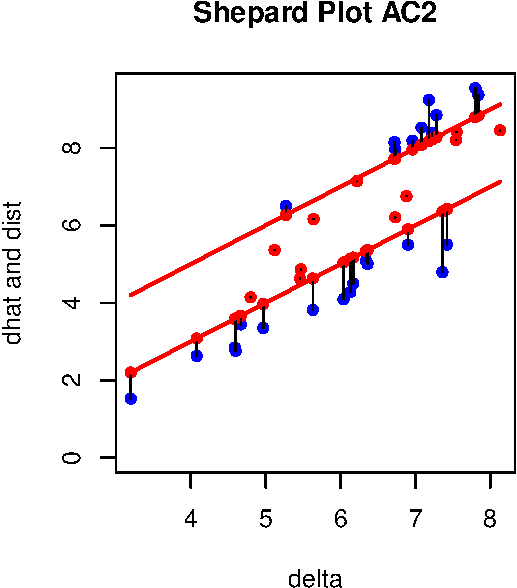
\includegraphics{smacofAC_files/figure-latex/gruijterh01-1} \end{center}

\begin{center}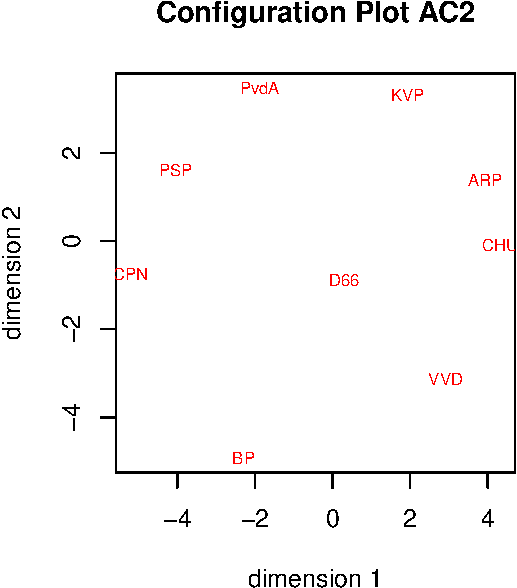
\includegraphics{smacofAC_files/figure-latex/gruijterh01-2} \end{center}

The bounds we use are \(\delta_{ij}\pm 1\). After 306 iterations
we arrive at stress \ensuremath{2.3629831\times 10^{-8}}. In the configuration plot the centrists
have moved to the center.
\#\# Type AC4

\begin{center}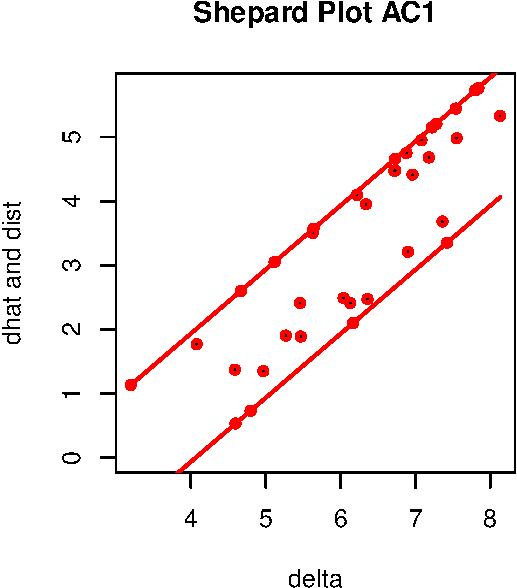
\includegraphics{smacofAC_files/figure-latex/gruijterh11-1} \end{center}

\begin{center}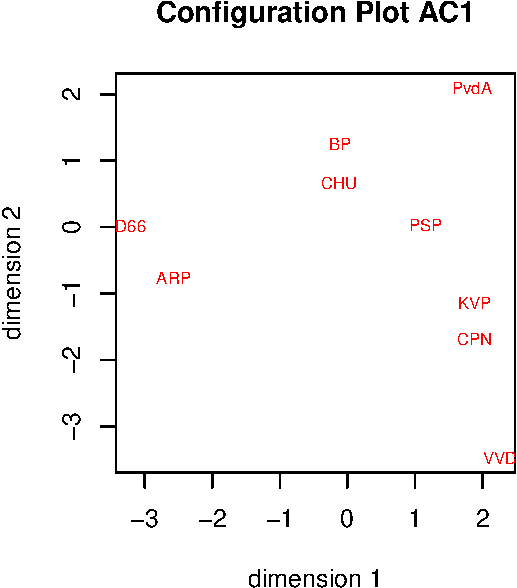
\includegraphics{smacofAC_files/figure-latex/gruijterh11-2} \end{center}

After 306 iterations stress is \ensuremath{2.3629831\times 10^{-8}}, i.e.~practically zero. We succeeded in moving all distances within the bounds. The additive constant is -3.0664907. The configuration
is again pretty much the same with D'66 in the center. VVD moves closer to the Christian
Democrats, and BP is more isolated.
\# References

\phantomsection\label{refs}
\begin{CSLReferences}{1}{0}
\bibitem[\citeproctext]{ref-cooper_72}
Cooper, L. G. 1972. {``{A New Solution to the Additive Constant Problem in Metric Multidimensional Scaling}.''} \emph{Psychometrika} 37 (3): 311--22.

\bibitem[\citeproctext]{ref-degruijter_67}
De Gruijter, D. N. M. 1967. {``{The Cognitive Structure of Dutch Political Parties in 1966}.''} Report E019-67. Psychological Institute, University of Leiden.

\bibitem[\citeproctext]{ref-deleeuw_stoop_A_84}
De Leeuw, J., and I. Stoop. 1984. {``Upper Bounds for Kruskal's Stress.''} \emph{Psychometrika} 49: 391--402.

\bibitem[\citeproctext]{ref-ekman_54}
Ekman, G. 1954. {``{Dimensions of Color Vision}.''} \emph{Journal of Psychology} 38: 467--74.

\bibitem[\citeproctext]{ref-heiser_91}
Heiser, W. J. 1991. {``{A Generalized Majorization Method for Least Squares Multidimensional Scaling of Pseudodistances that May Be Negative}.''} \emph{Psychometrika} 56 (1): 7--27.

\bibitem[\citeproctext]{ref-messick_abelson_56}
Messick, S. J., and R. P. Abelson. 1956. {``{The Additive Constant Problem in Multidimensional Scaling}.''} \emph{Psychometrika} 21 (1--17).

\end{CSLReferences}

\end{document}
